\chapter{Tecnologías Empleadas}

Debido a la facilidad de implementación y a sus ventajas, se ha empleado una arquitectura centralizada para el desarrollo del proyecto según se describe en \ref{2.3.1}. No obstante, sería interesante explorar soluciones distribuidas como posibles ampliaciones. 

En cuanto al procesamiento, transcodificación y entrega de video se probaron las tres alternativas mencionadas en \ref{2.2}. Para la solución propia se hizo uso de los servicios de Amazon Web Service con las tecnologías descritas en \ref{2.1}.

Para la creación de un Producto Mínimo Viable se ha decido implementar una página web debido a su facilidad de acceso desde cualquier dispositivo y a la adecuación de los \textit{frameworks} y tecnologías web a los objetivos del proyecto. Por ese motivo, a continuación se presentan las tecnologías utilizadas.


\section{Backend}

El backend es el conjunto de componentes que gestionan la lógica de negocio de una aplicación software, procesan datos, interactúan con la base de datos y administran la seguridad. Existe una amplia gama de tecnologías disponibles para seleccionar, especialmente en un entorno web. En esta sección, se analizarán las tecnologías preferidas y empleadas para la implementación de este servicio de streaming de videos en formato web.  

\subsection{TypeScript como lenguaje de programación}

TypeScript es un lenguaje de programación desarrollado por Microsoft y es una extensión de JavaScript. Lo especial de este es que incorpora tipado estático y mejores herramientas para detectar errores durante el desarrollo y no en producción. Esto ayuda a estructurar y crear proyectos software de forma más efectiva, permitiendo un mantenimiento del código más fácil.

En el caso del proyecto Booster, TypeScript resulta una herramienta útil debido a que el sistema integra múltiples capas de lógica como gestión de usuario, publicación y edición de metadatos de videos, autenticación, creación de comunidades y relación con la base de datos y el servidor. Por tanto, en este tipo de aplicaciones con un gran número de objetos de datos estructurados y bien definidos (usuario, videos, comunidades), el uso de tipado fuerte ayuda a reducir inconsistencias, detectar errores más fácilmente y mejorar la mantenibilidad del código. 

Más técnicamente, a diferencia de JavaScript, en TypeScript se pueden definir estructuras complejas y detectar errores de forma más clara. A modo de ejemplo, se pueden declarar variables de la siguiente forma:


\begin{lstlisting}[language=c]
    // con ':' se indica el tipo de la variable 
    //a diferencia de JavaScript donde solo se incluye un let. 
    saludos: string = "Hola"; 
    contador: number = 42;
    isFun: boolean = true;
    notas: number[] = [10,10,9.8];

    const user = {
        firstName: "Samuel",
        lastName: "Caraballo",
        role: "Autor",
    }

    
    console.log(user.name) // Property 'name' does not exist on type
                          //  '{ firstName: string; lastName: string; 
                          //role: string; }'.

\end{lstlisting}


De esta forma, se pueden detectar errores durante el desarrollo que por el contrario, serían más complejos de identificar. Es común, olvidarse del tipo de una variable e intentar hacer operaciones no permitidas para ese tipo. TypeScript, lo detecta automáticamente pero JavaScript, no es consciente de esto y en consecuencia se generan errores difíciles de detectar.  

\begin{figure}[h]
  \centering
  
\includegraphics[width=0.2\linewidth]{portada/typescript.png }
  \caption{Logo de TypeScript}
\end{figure}

\pagebreak
\textbf{Ventajas}

Su principal ventaja es la detección temprana de errores. Esto es importante en proyectos con una base de código grande, donde un pequeño fallo en la estructura de datos puede provocar errores más importantes y arruinar el servicio. 

Asimismo, el uso de typescript mejora la escalabilidad del proyecto permitiendo mantener un código más consistente y legible. 

El uso de TypeScript es importante en la industria y por esa razón, tiene una gran integración con herramientas modernas de desarrollo de aplicaciones web como Next.Js, Drizzle, tRPC, entre otros. 

\textbf{Desventajas}

Emplear TypeScript, requiere destinar más tiempo a la definición de tipos, lo cual incrementa el tiempo de desarrollo porque requiere mantener precisión y consistencia en todo el proyecto. Por tanto, esto añade complejidad adicional en comparación con JavaScript.

\textbf{Uso de Typescript}

TypeScript, se ha consolidad como una de las tecnologías más utilizadas en el desarrollo web actual. Es el lenguaje por excelencia para la capa \textit{backend} en plataformas SaaS, redes sociales y otras aplicaciones. La necesidad de compartir modelos de datos es un requerimiento frecuente en proyectos grandes y que utilizan tecnologías modernas como React.Js, Next.Js, Node.js, Express, entre otros. 

En Booster, al ser un proyecto de código abierto, TypeScript se emplea como lenguaje principal de programación para la integración de las distintas tecnologías, garantizar precisión y consistencia, detectar errores tempranos, mejorar la mantenibilidad y mantener la coherencia entre \textit{backend} y \textit{frontend}. 
\subsection{Base de Datos}

La base de datos es uno de los componentes más importantes en las aplicaciones software. Esto se debe a que constituye el sistema encargado de almacenar, consultar y actualizar la información del servicio. Para los objetivos de Booster, la base de datos debe permitir realizar consultas complejas de forma eficiente, integrarse con tecnologías modernas y soportar funcionalidades avanzadas como embeddings para implementar la búsqueda semántica de videos. 

Por estas razones, Booster integra una base de datos \textbf{PostgreSQL} como sistema principal. Este es un gestor de base de datos relacionales ampliamente utilizado en aplicaciones de todo tipo. Su funcionamiento está basado en el modelo relacional, donde la información se ordena y almacena en tablas, filas y columnas. Las relaciones, se modelas mediante claves primarias y foráneas. Este enfoque es el más adecuado para Booster ya que la información de usuarios, videos, comunidades es claramente estructurada. Además, este gestor de base de datos ofrece una gran cantidad de funcionalidades avanzadas, integridad referencial, un gran rendimiento en producción y una buena escalabilidad.


\begin{figure}[h]
  \centering
  
\includegraphics[width=0.4\linewidth]{portada/PostgreSQL.png }
  \caption{Logo de PostgreSQL}
\end{figure}

\textbf{Uso de PostgreSQL - NeonDB}

En Booster, PostgreSQL se integra a través de una plataforma de base de datos moderna y serverless diseñada para la nube conocida como \textbf{NeonDB}.

NeonDB presenta una arquitectura que separa almacenamiento y cómputo para ofrecer un escalado más flexible y administrar mejor la base de datos. Además, está especialmente diseñada para soportar funcionalidades de \textbf{Inteligencia Artificial}. En el caso de Booster, se han empleado extensiones como \lstinline|pgvector| para almacenar embeddings y realizar búsquedas semánticas de los títulos y descripciones de los videos. \cite{pgvector} Esta capacidad, permite realizar búsquedas más inteligentes en comparación a las búsquedas literales. Con esto, se puede encontrar contenido relacionado por significado y mejorar el sistema de recomendación ante una búsqueda en lenguaje natural. 


\begin{figure}[h]
  \centering
  
\includegraphics[width=0.4\linewidth]{portada/neondb.png }
  \caption{Logo de NeonDB}
\end{figure}

\textbf{Ventajas}

Implementar una base de datos PostgreSQL tiene diversas ventajas. Entre ellas, destaca la facilidad de administración. NeonDB ofrece un entorno gráfico para realizar consultas, ver los datos, tener un diagrama de la base de datos, entre otras funcionalidades que mejoran la gestión. Asimismo, PostgreSQL posee una documentación extensa y una gran compatibilidad con distintos ORMs y frameworks \textit{backend}.

\textbf{Desventajas}

Aunque es muy versátil, cuando hay un volumen alto de datos se requiere un diseño cuidadoso y un mantenimiento constante, incrementando el esfuerzo de desarrollo y la complejidad. Con un flujo de datos grande, es necesario incluir índices y destinar más tiempo a realizar optimizaciones lo que puede requerir más recursos técnicos. 

\pagebreak

\textbf{SupaBase}

De forma complementaria a NeonDB, se utiliza \textbf{SupaBase}, otra plataforma de \textit{backend} que implementa una base de datos PostgreSQL. Más concretamente, en Booster se hace uso de esta para implementar funcionalidades de chat en tiempo real. SupaBase Realtime permite transmitir eventos mediante WebSockets y estar pendiente a cambios en la base de datos en tiempo real, haciéndolo ideal para implementar chats en los canales para que sus seguidores puedan interactuar entre ellos y directamente con los creadores de contenido. 

\begin{figure}[h]
  \centering
  
\includegraphics[width=0.4\linewidth]{portada/supabase.png  }
  \caption{Logo de SupaBase}
\end{figure}



\subsection{ORMs}

Los ORMs (Object-Relational Mappers) son herramientas que permiten la interacción con bases de datos relacionales haciendo uso de estructuras del lenguaje de programación, en el caso de este proyecto, TypeScript. En lugar de depender exclusivamente de consultas SQL manuales, se implementan funciones que actúan como capa de abstracción y además mejoran la seguridad. Por tanto, el programador puede definir relaciones y transacciones directamente desde el código de la aplicación sin trabajar con filas y tablas SQL en cada operación.  

El uso de ORMs es muy común en aplicaciones modernas y existen un gran número de tecnologías a elegir. En este proyecto se han considerado dos: Drizzle y Prisma. Siendo la primera, la opción elegida para el desarrollo. 


\subsubsection{Drizzle}
Drizzle ORM \cite{drizzle} es un ORM orientado al desarrollo con TypeScript caracterizada por ofrecer una experiencia similar a SQL y tipada. 

Drizzle permite definir el esquema de la base de datos con código TypeScript mediante un archivo llamada \lstinline|schema.ts|. A partir del misommo, un desarrollador es capaz de establecer relaciones entre tablas y definir los tipos de datos de las columnas para realizar consultas tipadas. Además, permite combinar consultas SQL en sus funciones haciéndolo útil para consultas complejas y con varios pasos. 

La herramienta es ideal para el proyecto Booster. Esto se debe a que Drizzle permite realizar consultas avanzadas y específicas sobre bases de datos PostgreSQL.

\pagebreak

\textbf{Ventajas}


Su principal ventaja, es su tipado fuerte. Junto a TypeScript, ayuda a detectar errores durante el desarrollo y mantener la coherencia y precisión entre el esquema de base de datos y el \textit{backend}. A su vez, ayuda a prevenir inyecciones SQL mediante su capa de seguridad y mejores prácticas. 

Por otra parte, según lo menciona la documentación, tiene un diseño ligero y eficiente lo cual es favorable para el rendimiento de la aplicación. 

\textbf{Desventajas}

Drizzle es una herramienta nueva y además tiene una curva de aprendizaje elevada. Esto se debe a que requiere conocer bien el lenguaje SQL y tener experiencia con bases de datos relacionales antes de entender el funcionamiento del nivel de abstracción ofrecido por esta herramienta. Ofrece más control pero demanda un conocimiento técnico y completo.

\textbf{Uso de Drizzle}

En Booster se utiliza Drizzle como el ORM principal para interactuar con la base de datos. Una de las razones principales de esta elección es debido a que con un solo archivo \lstinline|schema.ts| se puede definir el esquema de la base de datos. Esto facilita la creación de tablas y relaciones y permite mantener la coherencia en todo el proyecto. Además, otro punto fuerte es su compatibilidad con las tecnologías empleadas y su capa extra de seguridad incorporada.

\begin{figure}[h]
  \centering
  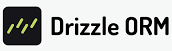
\includegraphics[width=0.4\linewidth]{portada/drizzle-orm.png }
  \caption{Logo de Drizzle-ORM}
\end{figure}



\subsubsection{Prisma}

Prisma es otro ORM popular en el desarrollo de aplicaciones TypeScript. El desarrollador define un esquema propio a partir del cual se genera un cliente TypeScript que se emplea para interactuar con la base de datos. En consecuencia, se consiguen realizar consultas con un gran soporte de auto-completado y con una sintaxis orientada al programador. Prisma destaca por su facilidad para modelar la base de datos incluyendo relaciones, entidades y operaciones comunes, así como también, su experiencia de uso. 

Es una buena opción cuando se necesita entregar un producto rápido y se busca legibilidad y tener una amplia variedad de herramientas adicionales. No obstante, para el proyecto se ha optado por Drizzle ya que esta tiene una relación más directa con SQL y es más ligera, mejorando así el rendimiento de la aplicación. 

Esta alternativa se menciona como una herramienta importante que se podría haber incluido y se evaluó antes de comenzar el desarrollo pero, no forma parte del \textit{backend} del proyecto final construido. 

\subsection{Comunicación Cliente Servidor - tRPC}

La comunicación cliente-servidor es esencial dentro de cualquier aplicación web moderna. En la plataforma Booster, esto permite que el \textit{frontend} se comunique con el \textit{backend} para recuperar datos, actualizarlos y ejecutar funciones como registro de usuario e inicio de sesión. Existen diversos enfoques, siendo APIs Rest o GraphQL las más conocidas. Sin embargo, para los efectos del proyecto se ha optado por una tecnología llamada \textbf{tRPC}. Esta, está orientada al desarrollo de RPCs (Remote Procedure Calls) con TypeScript que permite construir procedimientos de comunicación entre cliente y servidor respetando los tipos y garantizando coherencia y consistencia.

\textbf{tRPC} es una de las tecnologías fundamentales en este proyecto facilitando el intercambio de datos entre cliente y servidor. A diferencia de un enfoque REST, con tRPC se definen procedimientos en el servidor y el cliente se encarga de consumirlos sin necesidad de especificar un esquema de endpoints o capas adicionales de generación de tipos. Además, la utilización de esta biblioteca mejora la seguridad y la coherencia de tipos de extremo a extremo. Es decir, un tipo definido en el \textit{backend} se pueden compartir fácilmente hacia el \textit{frontend}, convirtiéndola en una herramienta ideal para el desarrollo \textit{full-stack}.

Al trabajar con tRPC es conveniente distinguir los siguientes conceptos. \cite{trpc-concepts}

\begin{itemize}
  \item \textbf{Procedure}:  un \textit{endpoint} de una API. Representa una acción concreta clasificadas en: consultas, mutaciones o suscripciones.  
  \item \textbf{Query}: Un procedimiento que obtiene datos.
  \item \textbf{Mutation}: Un procedimiento que modifica datos (create, update, delete).
  \item Suscripción: Un procedimiento que crea una conexión persistente y escucha cambios.
  \item \textbf{Router}: Un conjunto de procedimientos agrupados por un nombre. Por ejemplo la acción de modificar un video (updateVideo) está dentro de un router de videos que contiene más operaciones relacionadas con esa entidad. Por lo general, se suele tener un router por cada entidad en la base de datos.
  \item \textbf{Contexto}: Todo aquello accesible por un procedimiento. Usado normalmente para sesiones de estado de usuarios o conexiones a bases de datos.
  \item  \textbf{Middleware}: Una función que puede ejecutar código antes que se realice un procedimiento. 
  \item \textbf{Validación}: Verifica que los datos de entrada a un procedimiento cumplen con ciertas normas y son correctos.
\end{itemize}


\begin{figure}[h]
  \centering
  
\includegraphics[width=0.4\linewidth]{portada/trpc-logo.png}
  \caption{Logo de tRPC (typescript Remote Procedure Calls)}
\end{figure}


Lo particularmente interesante de tRPC es su integración con \textbf{TanStack Query} en el cliente lo cual añade mejoras de optimización, caché, revalidación, manejo de estados de carga y error, entre otras herramientas para mejorar la experiencia de uso. Esta es una de las principales razones por las que se emplea esta tecnología, además de su integración con typescript y otras tecnologías web.

\textbf{\textit{prefetch} con tRPC}

Este es el concepto (o método) más poderoso que tiene tRPC. Gracias a él, la experiencia de usuario se ve mejorada y los tiempos de carga reducidos. 

El \textit{prefetch} consiste en cargar datos por adelantados antes de que el cliente los necesite. En la figura, se observa el flujo de esta operación implementada en el proyecto.

\begin{figure}[h]
  \centering
  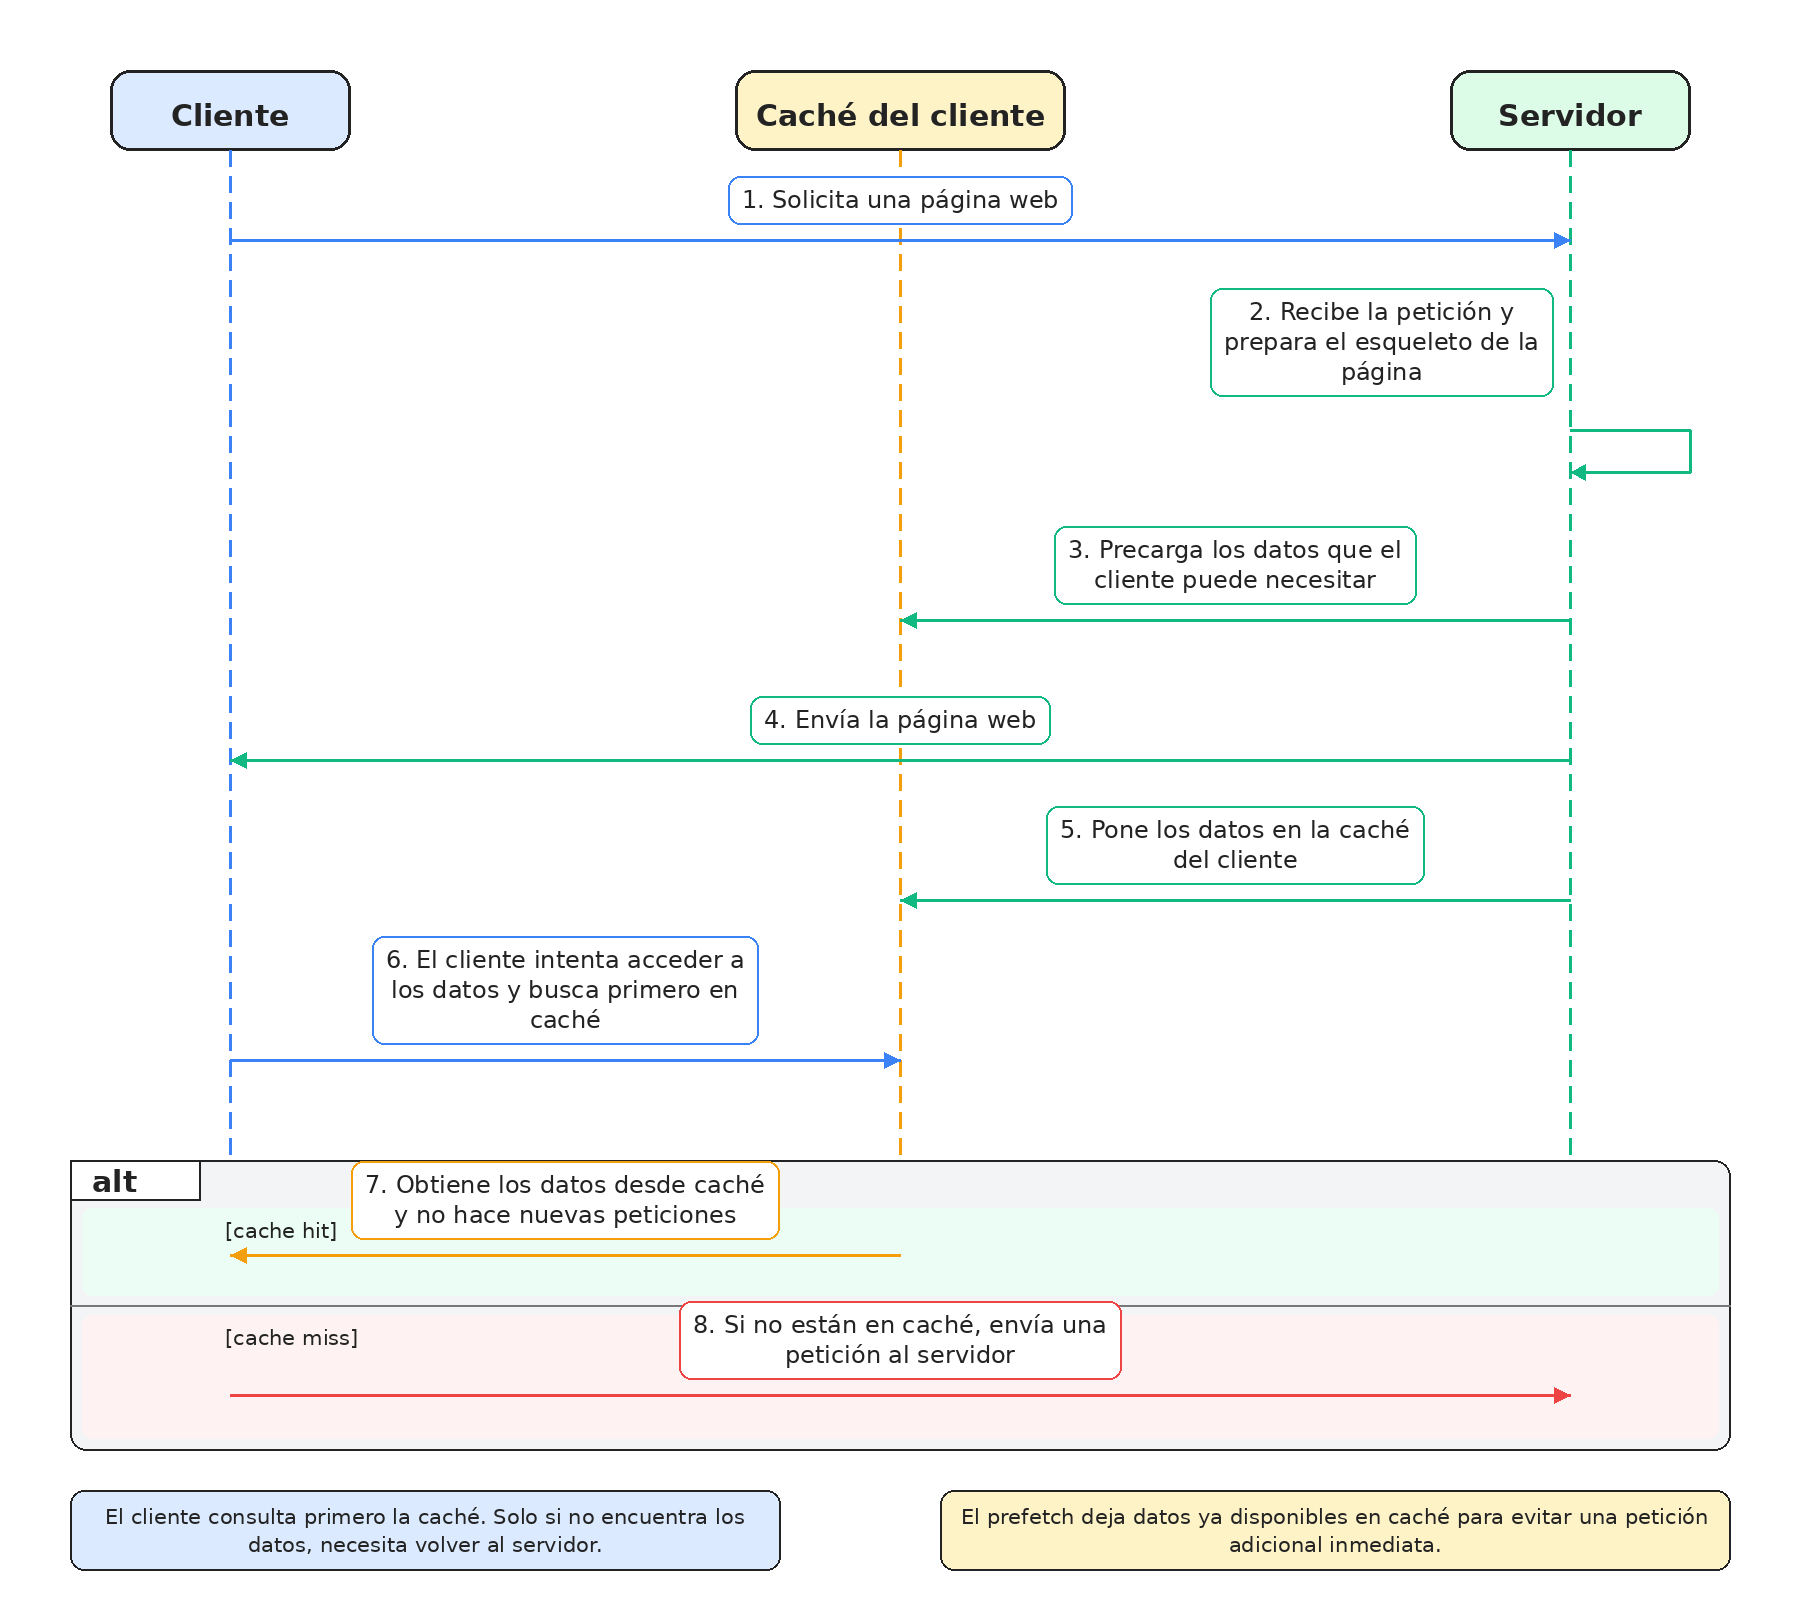
\includegraphics[width=1\linewidth]{portada/prefetch-diagram.png}
  \caption{Diagrama de secuencia de un flujo de \textit{prefetch}}
\end{figure}

Existen varias formas de aplicar el \textit{prefetch}. En el desarrollo de esta plataforma se ejecuta una pre-carga en el servidor antes de renderizar la página para que los datos estén disponibles cuando llegue al cliente. En Booster, esta técnica tiene un gran valor. Los usuarios están constantemente navegando entre listados de video, usuarios o comentarios por tanto, si los datos se cargan anticipadamente, el tiempo de espera disminuye creando la apariencia de una interfaz reactiva e inmediata. De esta forma tRPC tiene un doble uso: capa tipada de comunicación y un 'acelerador' de la interfaz de usuario. Por estas razones, se ha decidido utilizar tRPC para la comunicación cliente-servidor. 

\subsection{Next.js - backend}

\textbf{Next.js} es, junto con tRPC otra de las tecnologías fundamentales de este proyecto. Este es un framework de desarrollo web basado en \ref{React.Js} que permite construir aplicaciones \textit{full-stack} modernas, gestionando la interfaz de usuario y la lógica de negocio dentro de un mismo repositorio. En Booster, Next.Js se emplea para cumplir ambos de estos propósitos. Por un lado, se aprovechan sus habilidades de \textit{frontend} pero también, se hace uso de sus capacidades de backend facilitando la experiencia de desarrollo. 

Desde un punto de vista más técnico, para este proyecto se está empleando la versión moderna de Next.js que está basada en un \textbf{\textit{App Router}}. Este es un sistema de enrutamiento basado en el directorio \lstinline|/app|, en donde se gestionan las rutas de forma más eficiente. 
Es importante distinguir los siguientes conceptos:

\begin{itemize}
  \item \textbf{Server Component}: Es un componente de \ref{React.Js} que se ejecuta y se renderiza \textbf{únicamente} en el servidor. Por tanto, pueden acceder directamente a recursos del \textit{backend}.
  \item \textbf{Client Component}: Es un componente que se ejecuta solamente en el cliente (navegador). Normalmente, se suele reservar para interacciones con la interfaz de usuario donde la disposición de la página web puede variar.  
\end{itemize}

Durante el desarrollo de Booster se combinan las habilidades de los Server Components y los Client Components para mejorar la eficiencia y optimizar el rendimiento de la aplicación. Por otra parte, gracias al \textit{App Router} \cite{nextjs-app} se logran crear manejadores personalizados de peticiones HTTP, rutas de APIs estáticas y dinámica y crear queries de consulta. Todo esto se puede conseguir sin la necesidad de un servidor \textit{backend} separado lo cual facilita el desarrollo y ayuda a mejorar la coherencia en la aplicación. 

En Booster, esto es extremadamente útil ya que permite concentrar en un mismo entorno diversas responsabilidades. Next.Js se encarga de mostrar la aplicación, gestionar la obtención de datos, la comunicación cliente-servidor junto con tRPC y definir rutas de API y direcciones URL. 

Además Next.Js contiene métodos de optimización como: incorporación de cachés, revalidación, pre-carga de enlaces, optimizaciones de imágenes, optimizaciones de código css \todo{Poner ref a CSS, tailwindcss} y optimizaciones de navegación. 

\textbf{Ventajas}

Su principal ventaja es su integración \textit{full-stack}. Se puede desarrollar el cliente y el servidor en un mismo repositorio facilitando el proceso de desarrollo y despliegue. Además, emplea reglas, formatos y mejores prácticas que simplifican  la creación de aplicaciones web. Su integración con TypeScript y otras herramientas modernas lo convierte en una opción ideal para Booster. 

Contiene una gran variedad de elementos de optimización para mejorar el rendimiento de la aplicación. En una plataforma como Booster, esto es importante ya que mejora la experiencia de usuario de forma significativa. 

Otro aspecto importante a destacar es que como Next.Js utiliza pre-renderizado estático (Static Site Generation SSG) \footnote{Se entiende por pre-renderizado estático (SSG) a aquel proceso de generación de páginas HTML en el momento de construcción (build time). Se ejecutan comandos como \lstinline|npm run build| para generar archivos estáticos (.html, .css, .js) y de esta forma, estas páginas cargan de forma instantánea al no necesitar un servidor para solicitar datos}, \todo{poner ref o citar a mas info} los motores de búsqueda pueden indexar de forma más sencilla el contenido de la página web. Así, se consigue mejorar su descubrimiento en internet e incrementar el tráfico: Se mejora el Search Engine Optimization (SEO)

\textbf{Desventajas}

Al concentrar \textit{frontend} y \textit{backend} en un mismo lugar, la complejidad de los proyectos suele considerar de forma considerable. 

Otro aspecto importante a mencionar es su elevada curva de aprendizaje. Con los años se han añadido un gran número de operaciones y optimizaciones incrementando la cantidad de conceptos y técnicas lo que puede resultar dominar Next.Js en una tarea más difícil. 










\section{Frontend}

\subsection{React.Js}
\label{React.Js}

\subsection{Next.Js - frontend}

\subsection{Tailwindcss y Shadcn}